\documentclass[../main/main.tex]{subfiles}

\newdate{date}{13}{05}{2020}

\begin{document}

\section{Lecture 19}
 \displaydate{date}. Compiled:  \today. Martina 
 
 
\subsubsection{Slide 309}

\begin{figure}[h!]
\centering
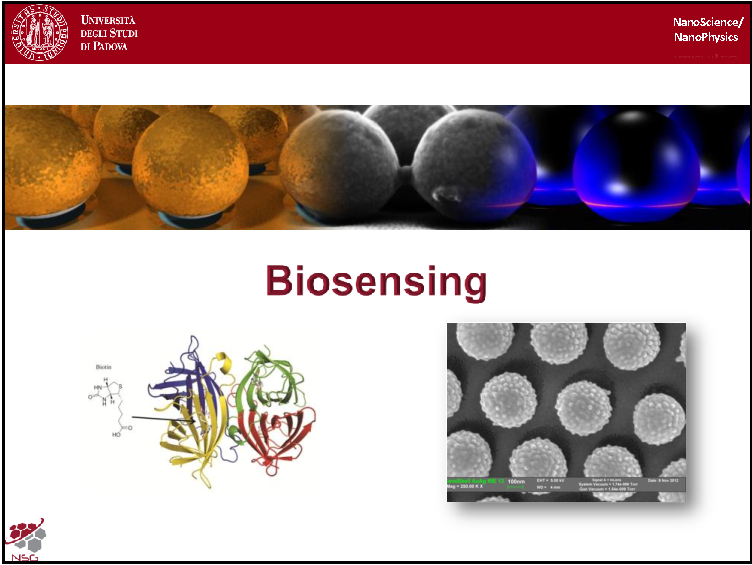
\includegraphics[page=1,width=0.9\textwidth]{../lessons/pdf_file/19_lesson.pdf}
\end{figure}

As we have seen interacting nanostructures are better for enhancing the optical properties due to the enhanced local field amplification between two neighbour NP, as we have seen for the non-linear optical properties activated in a strong way for the nano-planar geometry.

In this lesson I would like to discuss another kind of application in which the interaction can be exploited to enhance the performances of a function of nanostructures in the interacting regime.

To do that I will briefly describe the biosensing application of plasmonic nanostructures made out of ordered arrays of semi-nanoshell, this 2D arrangement on a surface of a transparent substrate like silica or those peculiar structures here, and they can be set, ordered, and with a size of around $100 nm$ with tiny shell around a dielectric core, as we will see in a moment, which is able to tune the plasmonic resonances of these nanostructures in the near infrared regime.

This is a simulated image of the structure in terms of the metallic core, and this is a simulation of the near field enhancement in our structures, and we will try to see the effect of controlling the relative distance  between two neighbouring nanostructures to enhance the capability of these structures to probe concentration of recognition event, which is one of the most used probe receptor interaction and which can be exploited in a very effective way to test the performances of a biosensor.

\newpage

\subsubsection{Slide 310}

\begin{figure}[h!]
\centering
\includegraphics[page=2,width=0.9\textwidth]{../lessons/pdf_file/19_lesson.pdf}
\end{figure}

Just to better understand what is a semi-nanoshell array, let's see briefly what is it. To obtain a semi-nanoshell we can consider a dielectric core, that could be polystyrene NP, surrounded by a shell of a suitable plasmonic metal, in our case gold, since the deposition is done in a given direction, the coverage will be non-uniform, so we will obtain this non-uniform coverage which is very important for the performance because we will exploit a lateral interaction between such kind of nanoshell. 

In this core-shell system, if we look at the cross-section of course we have the dielectric core (which can be polystyrene or silica) and the shell (it can be any noble metal element, gold, silver, any alloy, or it could be a non-plasmonic metal, a transition metal). 

The idea is to arrange those NP in a 2D ordered array, so that we can control the lateral coupling between two nanostructures. As you can see the position is quite rough in the sense that it is not exactly a smooth surface, but the surface is made out of bumps, which can be helpful in creating even an additional structure in the hotspot for the local electric field. 

This is the scale in our system, which is $100 nm$, so typically those structures are  $200/300 nm$ in diameter, but it can be controlled in a very wide range of sizes, with a tiny shell of few tens of nanometers in the highest thickness in our system.

\newpage

\subsubsection{Slide 311}

\begin{figure}[h!]
\centering
\includegraphics[page=3,width=0.9\textwidth]{../lessons/pdf_file/19_lesson.pdf}
\end{figure}

So, let's see how we can produce that. We can use what is called the nano-sphere lithography. The nano-sphere lithography is a kind of lithographic approach in which we use a mass deposition with polystyrene nanosphere with size which can be tuned but the range is very wide, we can go even lower than this value, they are monodispersive, they are conventional nanostructures, NP, so they can be obtained in a very controlled way, and with this technique we can make them self assemble in a mono-layer ordered as you can see in this electron microscope here, with a close packed hexagonal geometry, so that you can have an attaching nanosphere of polystyrene and basically this is sort of structures which is able to interact with light in a very clever way, so that it produces this change of local colour, those are substrates with deposited nanosphere, one mono-layer of those NP and you can see that you can easily obtain centimeter squared arrays of those ordered mono-layers, which can be used to produce ordered 2D nanostructures.

\newpage

\subsubsection{Slide 312}

\begin{figure}[h!]
\centering
\includegraphics[page=4,width=0.9\textwidth]{../lessons/pdf_file/19_lesson.pdf}
\end{figure}

After performing the synthesis of the 2D mono-layer of ordered NP of polystyrene, we perform Reacting Ion Etching process which is a sort of physical chemical etching step in which we use a mixture of oxygen and argon gases to chemically and physically modify the polystyrene NP without affecting the center to center distance but just reducing the size of the polystyrene nanospheres.

We do that exploiting the oxidation effect of oxygen which is able to chemically interact and decompose the surface of the polystyrene particles, coupled with argon which is able to provide kinetic energy to remove the new species produced at the surface, so that the net effect is to produce a reduction in size and also modification in the shape of the nanospheres as we can see in this cross-section SEM image and you see that we go from a spherical polystyrene nanospheres into this lens-like object and this is due to the anisotropic effect of this reactive ion etching which is strongly directional in this range here, so we are able to reduce this size, but without affecting the holder of the NP.

This rough surface is the product of the combination of the chemical and physical etching of the surface. You can control the degree of roughness of the surface by enhancing or decreasing the partial pressure of argon in the system. 

This is just a technicality, but what is important i that we are now able to obtain nanospheres or nanolenses in which there is no lateral contact between neighbouring nanoobjects. 

\newpage

\subsubsection{Slide 313}

\begin{figure}[h!]
\centering
\includegraphics[page=5,width=0.9\textwidth]{../lessons/pdf_file/19_lesson.pdf}
\end{figure}

Then we perform the deposition of the metal, we use for instance gold to decorate the particles, so you can tune the thickness of the metallic deposition, so that you can further control the level of lateral coupling between the 2D nanostructures.

With this lateral control we can obtain a very interesting platform for sensing, because we can exploit the linear optical properties, the surface plasmon resonance of these NP in the interacting regime, because in this case of course we cannot neglect the interaction between neighbour NP.

And this is the lateral view of the nanostructures, ordered with this peculiar shape of the metallic decoration.

\newpage

\subsubsection{Slide 314-315}

\begin{figure}[h!]
\centering
\includegraphics[page=6,width=0.9\textwidth]{../lessons/pdf_file/19_lesson.pdf}
\end{figure}

\begin{figure}[h!]
\centering
\includegraphics[page=7,width=0.9\textwidth]{../lessons/pdf_file/19_lesson.pdf}
\end{figure}

If we want to build a plasmonic sensor out of a single noble metal NP sphere made out of gold or silver or whatever is the element, we can exploit the surface plasmon resonance which is described by the localized SPR Fr\"olich condition for the resonance in the visible range.

We know that it depends on a lot of properties but in particular it strongly depends on the surrounding medium, because this dielectric function can be modified by modifying the medium around the NP, but of course if we want to change the optical properties and to use NP as transducers, if we are able to produce a dielectric shell made out of the material that we want to probe, which is able to selectively attach to a probe at the surface of the NP, we are able to obtain a core-shell system which is in this case very easy to be modeled, in the case of semi-nanoshell not that easy because of the shape and anisotropy in the metal distribution, but in principle the effect is the same, so the presence of this dielectric shell around the particle, which resembles for instance the effect of biological molecules around the NP of course we expect a redshift of the resonance due to this local increasing of the dielectric refractive index, so that we can transduce a dielectric change into an SPR change which can be recast in terms of a selective measurement of the concentration of the molecules which produce the dielectric shell around our system, so that we can obtain the output signal of our sensor, which is an optical sensor.

\newpage

\subsubsection{Slide 316}

\begin{figure}[h!]
\centering
\includegraphics[page=8,width=0.9\textwidth]{../lessons/pdf_file/19_lesson.pdf}
\end{figure}

The typical system that is used to test the capability of an optical system to be used as biosensor is this scheme Biotin-Streptavidin recognition and in this case Biotin is a tiny molecule with a very light molecular weight with respect to the much larger Streptavidin molecule which is quite large and which has four lobes which are able to selectively bind to Biotin for which it has very high affinity, so for that reason this is used to control the performance of a biosensor.

The Streptavidin acts as the analyte, that is the molecule you want to probe and the Biotin will act as the receptor, which is the molecule that we attach to the surface f our system because this is a Biotin with thiols at the end, that is this sulfur atom which is able to selectively bind with a covalent bond to the surface of the metallic structure, in order to perform this binding and decoration of a NP which is decorated by a uniform layer of receptors.

Of course we can tune the relative distance between the Biotin molecules by adding suitable spacers.

\newpage

\subsubsection{Slide 317}

\begin{figure}[h!]
\centering
\includegraphics[page=9,width=0.9\textwidth]{../lessons/pdf_file/19_lesson.pdf}
\end{figure}

For instance if we imagine this to be the surface of our nanostructure, the metallic nanostructure, what we normally do is to make first a self-assembled mono-layer of thiols by mixing two kind of thiols, and some of them exhibit a molecule which is able to bind to the Biotin and others are not, so that we can obtain a sort of statistically spacing of our molecule, which are the ones able to bind to the Biotin which are the Mercaptoundecanoic acids spaced by the Octanethiol system which is this molecule here.

After that we need to immobilize the Biotin which is Biotin with a PEG molecule attached and with an Amine group attached, which is able to interact with the Carboxile group of the Mercaptoundecanoic acids, so that to form the binding, so that in the end we are able to immobilize the Biotin molecule just on the Mercaptoundecanoic acid once, so that with a given controlled spacing in order to let enough space for the largest Streptavidin molecule to arrive and to attach to the Biotin molecule.

The analyte, in this case the Streptavidin, so if we expose our sensors to the solution which we set different concentration of the Streptavidin, so that we are able to measure the plasmonic shift as a function of the concentration of this Streptavidin, using the selective binding of Streptavidin to the Biotin, we know that the modification of the dielectric properties around NP is due to this selective interaction.

This is why we say that this sensor is a selective sensor, because if we add other molecules which are not able to bind to Biotin, that would not selectively attach, so that they will not produce the modification of the dielectric function at the surface of the structures. 

In general this object can be described by an effective layer of thickness around $4/5 nm$ in size at most, with an equivalent dielectric function around $1.5$ squared, thus the refractive index of this layer is around $1.5$, which as I mentioned is a typical refractive index of biological related structures.

After that we can measure the redshift of the optical signal in our system upon the recognition of the Streptavidin.

\newpage

\subsubsection{Slide 318}

\begin{figure}[h!]
\centering
\includegraphics[page=10,width=0.9\textwidth]{../lessons/pdf_file/19_lesson.pdf}
\end{figure}

Just to report some results here, we explored two configurations of nanospheres. The one with low interaction,that is nanostructures well spaced with a gap sufficient to have a decay of the local field so that the interaction can be safely neglected, this situation here, and another with a very high interaction in which the gap is of few nanometers statistically so that we have from one side the isolated structures, this one of low interaction nanostructures, with the resonance around $120 nm$ in wavelength, so we are in the infrared, and thy interacting configuration around $1200 nm$ in wavelength.

As expected the interacting configuration shifts to higher in wavelength or lower interaction as we described in the hybridization scheme for the interaction.

\newpage

\subsubsection{Slide 319}

\begin{figure}[h!]
\centering
\includegraphics[page=11,width=0.9\textwidth]{../lessons/pdf_file/19_lesson.pdf}
\end{figure}

And performing the functionalization as we have seen in the previous steps, we obtain a step by step variation of the peak resonance with just looking at the surface plasmon resonance just to see the tiny shifts produced by the molecules and we were able to follow all the steps of the functionalization and by measuring this shift we were able to obtain curves like this one in which we report the concentration of the Streptavidin in the solution in molar units.

\newpage

\subsubsection{Slide 320}

\begin{figure}[h!]
\centering
\includegraphics[page=12,width=0.9\textwidth]{../lessons/pdf_file/19_lesson.pdf}
\end{figure}

As you see the range that can explore with those biosensors goes down to $10^{9-} M$ which is $nM$ or even we can reach the range of $pM$ like in this case, and we can clearly see that the interacting configuration, that is the blue line, is able to produce a larger shift for the very same level of concentration, and this is due to the local field amplification in the nanostructures. 

We are able to obtain what is called LOD, which is the limit of detection of our system, which is of the order of $10^{-11}/10^{-10} M$, which is remarkably low amount of molecules probed by this optical sensors, so you can easily obtain early stage recognition of possible other molecules expressed by given diseases in the human body, so those results are very promising for obtaining what is called label-free plasmonic sensors, it means that you do not need to attach any fluorescent label to the molecules that you want to probe to be used as in old-fashion fluorescent sensors in which you were measuring the fluorescence coming from labels attached to the probe, this complicates a lot the chemistry that you need to have to obtain such a sensor.

In our case we directly produce the recognition by suitably attaching a probe at the surface of our nanostructure and measuring the binding event through this redshift of the surface plasmon resonance.

We fitted in this semi-logarithmic scale the evolution of the performance of our structure whit what is called Langmuir Isotherm, which is a typical function that is used to describe phenomena related to the binding event of a couple of molecules, with affinity constant $K_a$ with a concentration $[SA]$, which is the concentration of the Streptavidin in our case, and this is the typical evolution of our structures.

Of course we measured this function here, and if we know the concentration we can obtain information on the saturation value of the maximum shift that we can obtain with our system, that is when we saturate all the Biotin probes with the Streptavidin so additional Streptavidin cannot be probed but of course this occurs at very high concentration so there is no need of this specialized technique for us to assign the concentration, and we can obtain information on the affinity constant or the effective affinity constant of our specific binding which is normally expected to be lower then the nominal affinity constant of Biotin-Streptavidin in liquid, because in that case the two molecules are able to bind with any other spatial constraint, in this case we are at the surface of the NP, we have a lateral entrance of the neighbouring Biotin molecules.

\newpage

\subsubsection{Slide 321}

\begin{figure}[h!]
\centering
\includegraphics[page=13,width=0.9\textwidth]{../lessons/pdf_file/19_lesson.pdf}
\end{figure}

As we have seen the interaction between NP can be very effectively controlled in the performances of our nanosystems in actual devices and we have seen for the non-linear optical applications, for the biosensors applications. Of course at this point the problem is how can we even improve those results by designing better and better structures in terms of the controlled interaction.

One interesting example of this kind of investigation is the one related to a peculiar kind of interacting NP and in particular the one which led to the idea of plasmonic nano-lenses in a similar configuration. 

\newpage

\subsubsection{Slide 322}

\begin{figure}[h!]
\centering
\includegraphics[page=14,width=0.9\textwidth]{../lessons/pdf_file/19_lesson.pdf}
\end{figure}

In this case what we want to do is the following: we want to exploit self-similarity as a way to selectively pump the local field by suitably coupling neighbouring NP arranged with respect to the size and distance in a way that we can build sort of self-similar transformation in the system to obtain the sequence of the NP. 

For instance instead of having a linear chain, as we have seen, with a similar or equal NP with equal spacing in which we have seen that the net effect in terms of the near field is not that dramatic by acting in increasing number of NP, in this case we want to suitably design the system in order to try to get the most out of the NP and this idea of asymmetric nano-lenses exploiting self-similarity was proposed in the early years of the century by Stockman and he proposed this structure in which the size is scaled by a factor $s$ with respect to the previous one and the relative distance is also scaled by the same factor, so that we have starting with a given size the next NP will have a reduced size and with respect to this distance, the next distance will be scaled by the very same scaling factor.

For instance they investigated the properties of the asymmetric nano-lenses for a particular value of $s$ which is $1/3$ in this case and for particular values of the number of NP which is $3$ with size decreasing from $45/50$ to $5 nm$ in radius, and with a given relative distance of $0.6$ with respect to the radius, that this automatically satisfies also this scaling law since it is attached to the size of the previous NP.

In order to have a first rough estimate of why this asymmetric nano-lenses are expected to produce an amplification in the field in this interacting NP configuration, we can do a very simple calculation based on some assumption, for instance if $s$ is much less than $1$ so that the particles are in a dipolar regime, with a strong interaction in the near field, and if we can use the dipolar approximation, we can immediately calculate what is the effect of the amplification of the near field by adding a sequence of NP, for instance for the first NP if we shine an electric field $E_0$ we know that we are in the independent particle approximation, so we can use the Mie theory in the dipolar approximation so we have the local field enhancement, if we are at the resonance for the particle we can include the Fr\"olich condition so that the local field enhancement is purely real at the resonance and it amounts to this factor here, which we have seen that for silver can be of the order of $10$ with respect to the external field.

But then we have a second NP here and if the system is still in the dipolar approximation we can obtain a gain that the near field amplification is nothing but the field produced by the first amplified by the local field enhancement of the second next NP which is still $f$, of course assuming that this is not strongly dependent on the size and for that reason we obtain this sequence, the local field of the second particle is amplified with respect to the one of the first particle by a factor $f$ that is  factor $f^2$ with respect to the external field.

If we continue we end up that the particle labeled with $n$ will have a local field amplification which is of the order of the local field enhancement at resonance elevated to the power of $n$ so that with $n$ equal $3$ we can expect $1000$ amplification of the field, which is much larger then the incoming electric field.

Of course for a clear symmetry reason the largest amplification is expected to occur in the region between the last two NP and this is why we use the rough estimate of $s<<1$ because we want to stay in the near field of the first particle in order to this approximation to hold, but of course this is just a rough estimate, we can do full electrodynamic calculation with the generalized multiparticle Mie theory of this nano-lenses to obtain real structures of the resonance.

Another important thing that we used for constructing this amplification is that the resonance of the NP is not dependent on the size, that is quite strong approximation because we have seen, that as a function of the size there could be variation if the dipolar approximation is no longer valid, but we will discuss briefly in the following this point. So for the moment let's use the Stockman self-similar nano-lens and try to see what is the actual field amplification in this point here and the result is reported in this picture here.

\newpage

\subsubsection{Slide 323}

\begin{figure}[h!]
\centering
\includegraphics[page=15,width=0.9\textwidth]{../lessons/pdf_file/19_lesson.pdf}
\end{figure}

This is the near field amplification in the equatorial plane of this structure, the red pint is the hotspot and as expected the hotspot at the resonance this particular nanostructure is found to be of the order of $1000$ which is exactly what we expected with respect to the isolated NP with silver the energy of the resonance at the surface plasmon is around $3.5 eV$ in vacuum, in the case of the nano-lens since we are in the interacting approximation, the resonance is slightly redshifted, that is at lower energy or at large wavelength as reported here, at $3.37 eV$. 

\newpage
\subsubsection{Slide 324}

\begin{figure}[h!]
\centering
\includegraphics[page=16,width=0.9\textwidth]{../lessons/pdf_file/19_lesson.pdf}
\end{figure}

Of course you can optimize this value but what is important to realize is that if you change the wavelength of the pumping field of course you will obtain a decreasing local field amplification in the case of our system, so that we end up in much lower field amplification, because it is a resonant process, the field amplification.

Of course this idea can be further optimized by changing the relative distance between the particles, the size, the number of particles, and I have to say that in the original paper of Stockman they used the dipolar approximation for he NP, so their calculation was not perfectly agreeable, but the main message of the nano-lenses is there and it is a very clever idea. Of course not that easy to be implemented in a simple nanofabrication technique because you need to produce very controlled positioning and sizing of the NP in order to exploit at the fullest this kind of structures.


\newpage

\subsubsection{Slide 325}

\begin{figure}[h!]
\centering
\includegraphics[page=17,width=0.9\textwidth]{../lessons/pdf_file/19_lesson.pdf}
\end{figure}

But of course if you think of an asymmetric nano-lens you can immediately generalize this concept to the symmetric version, why not adding a symmetric version of this lens in this region here, so that we can obtain a field amplification exactly in the middle and that was done by Stockman and coworkers and they tried to analyze this structure with a very same scaling law as before and they were able to obtain a even better results.

\newpage

\subsubsection{Slide 326}

\begin{figure}[h!]
\centering
\includegraphics[page=18,width=0.9\textwidth]{../lessons/pdf_file/19_lesson.pdf}
\end{figure}

The resonance did not shift substantially and the field amplification was almost rised by a factor $2$, so as expected we have a doubling of the local field enhancement and in this case of course again it is strong function of the wavelength because if we are out of the resonance of the system, the local amplification starts to decrease, but the idea of course is very clever also in this case, we have a symmetric position of the hotspot in this case because of the assumption in our system.

\newpage

\subsubsection{Slide 327}

\begin{figure}[h!]
\centering
\includegraphics[page=19,width=0.9\textwidth]{../lessons/pdf_file/19_lesson.pdf}
\end{figure}

An important question when dealing with surface plasmon resonance and enhancement linear field by interaction between neighbouring NP, is that it is easy to calculate the near field properties and it is easy as well to measure the far field properties, but  is it easy to measure or to have access to the near field properties of a nanostructures which is of paramount importance to decide if the structure is interesting or not in terms of possible specific application, as we have seen.

So the idea is, are we able to measure the near field properties of a plasmonic system interacting or not independently on the degree of interaction. 

\newpage

\subsubsection{Slide 328}

\begin{figure}[h!]
\centering
\includegraphics[page=20,width=0.9\textwidth]{../lessons/pdf_file/19_lesson.pdf}
\end{figure}

The answer is partially yes in the sense that if we want to have access to the near field properties we want to measure the light scattered by the particles, and the first technique that we may think of is the optical microscopy if we are dealing with SPR resonance. 

This is actually a very clever solution, of course the problem is that you do not have very high spatial resolution because you work with visible light, you know that the resolution of any optical system working at a given wavelength $\lambda$ is at most of the order of $\lambda/2$, which is the diffraction limit,after that the wave will be scattered and you cannot reconstruct the information with high enough accuracy to localize the source, producing this scattered light, but of course if you are able to control the position of your NP, you are able to obtain information on the local structure of single NP, like in this beautiful experiment with the so called Dark-field optical microscopy, in which you do not measure the standard total light emerging from the excitation with visible light of the NP but just the scattered light, for that reason we speak about dark-field microscopy and not bright-field microscopy like in the normal situation.

The image that you obtain as this one but the structure from which is obtained is of course measured by a much more sensitive technique like transmission electron microscopy which is able to produce subnanometer resolution, so if your structure is made out of NP, a colloidal solution of silver NP dispersed on a substrate which is in this case just a carbon foil, and if the separation between neighbour NP is sufficiently large with respect to the wavelength, so that we can spot individual NP of course we can measure what is called correlation microscopy, in which you can easily recognize the scattering from individual objects or scattering from couple of object because in this case two particles are so close that they scatter as a single object with respect to the dark-field microscopy which is not of course able to spot the relative distance between the two objects. 

So as I mentioned this technique is not able to spatially isolate the source of the light, but  if the source is already partially well resolved it is a very powerful technique. Indeed you see that the light emerging from different particles is of different colours, and these different colours mean that you can obtain information on the size dependent scattering with respect to the NP in our system. 

\newpage

\subsubsection{Slide 329}

\begin{figure}[h!]
\centering
\includegraphics[page=21,width=0.9\textwidth]{../lessons/pdf_file/19_lesson.pdf}
\end{figure}

Indeed if you closely look at what is the shape of that particular configuration which produces this light and if you spectrally analyze the light which here is reconstructed with the full colour, but it can be reconstructed by correlating the shape and the spectral position of the resonance like in this picture here, so you can clearly realize that different shape NP are able to produce resonances in different region of the spectrum, for instance if you go from spherical NP or toroidal NP of silver, you are more or less close to the $400 nm$ in wavelength, if you have this pentagon-like NP you have a redshift, if in this case you have triangular NP you have even larger redshift, and of course this is the scattered light, and you can clearly even see the variation of the scattering as a function of rounding the corners with respect to a perfectly triangular prism to rounded prism, to even more rounded prism of course. 

The close you get to a spherical particle, the blueshifted is the spectrum with respect to the system in which you have a sharp corners.

With this technique of course, provided that you are able to obtain isolated NP, you can obtain a very good way to verify the calculation model that you used to obtain a scattering properties of different reshaped NP, and we will see how to simulate different shapes with a given composition to predict with easy calculation the position of all those resonances in our system.

So, this technique is really very powerful but as I mentioned suffers this assumption that all the NP should be isolated, otherwise you cannot distinguish between the spectrum arising from neighbouring NP with respect to the on of truly isolated NP.





\clearpage


\end{document}